\documentclass[a4paper, 11pt]{report}% autres choix : book, report
\usepackage[utf8]{inputenc}% gestion des accents (source)
\usepackage[T1]{fontenc}% gestion des accents (PDF)
\usepackage[francais]{babel}% gestion du français
\usepackage{natbib}% utilisation du lib de référence zotero
\usepackage{textcomp}% caractères additionnels
\usepackage{mathtools,amssymb,amsthm}% packages de l'AMS + mathtools
\usepackage{lmodern}% police de caractère
\usepackage{geometry}% gestion des marges
\usepackage{graphicx}% gestion des images
\usepackage{caption}% gestion des figures
\usepackage{subcaption}% sous figures
\usepackage{xcolor}% gestion des couleurs
\usepackage{array}% gestion améliorée des tableaux
\usepackage{calc}% syntaxe naurelle pour les calculs
\usepackage{titlesec}% pour les sections
\usepackage{titletoc}% pour la table des matières
\usepackage{fancyhdr}% pour les en-têtes
\usepackage{titling}% pour le titre
\usepackage{enumitem}% pour les listes numérotées
\usepackage[hyphens]{url} % Pour des césures correctes dansles URLs
\usepackage[pdfauthor = {{MB TC AP}}, pdftitle = {{Modelisation Lokta Volterra}}, pdfstartview = Fit, pdfpagelayout = SinglePage , pdfnewwindow = true, bookmarksnumbered = true, breaklinks, colorlinks, linkcolor = black, urlcolor = black, citecolor = cyan, linktoc = all]{hyperref}
\usepackage{titlesec}

\titleformat{\chapter}[block]
  {\normalfont\Huge\bfseries}% font of number
  {\thechapter~ -}% format of number
  {20pt}% space between number and title
  {\Huge}% font of title
  
% Taille des marges
\geometry{hmargin=2.8cm,vmargin=2.8cm}

% RAZ des numéros de section après un chapitre
\makeatletter\@addtoreset{section}{chapter}\makeatother
% Pour mettre des I, II, etc. aux parties
\renewcommand{\thepart}{\Roman{part}}
% Pour mettre des 1, 2, etc. aux chapitres
\renewcommand{\thechapter}{\Roman{chapter}}
% Idem pour les sections et avoir le numéro de chapitre
\renewcommand{\thesection}{\Roman{section}}
% Idem pour les sous-sections et avoir le numéro de chapitre
\renewcommand{\thesubsection}{\Roman{section}.\arabic{subsection}}

\titlecontents{section}%
	[1.5em]% retrait à gauche
	{\addvspace{1em plus 0pt}\bfseries}% matériel avantcommun aux entrées numérotées ou pas
	{\contentslabel{2em}}% avant lorsqu'il y a un numéro
	{\hspace{-1.3em}}% avant lorsqu'il n'y a pas de numéro
	{\hfill\contentspage}% points de suspension et no page
	[\addvspace{0pt}]% matériel après
	
	\dottedcontents{subsection}%
	[4.5em]% retrait gauche
	{\addvspace{0pt}}% matériel avant
	{3em}% espacement de contentslabel
	{0.75em}% espace entre les . . . .
    [\addvspace{0pt}]% matériel après

    \dottedcontents{subsubsection}%
	[6em]% retrait gauche
	{\addvspace{0pt}}% matériel avant
	{3em}% espacement de contentslabel
	{0.75em}% espace entre les . . . .
    [\addvspace{0pt}]% matériel après

% En-tête, pied de page
\pagestyle{fancy}
\fancyhead[O]{Mini-Pojet \\Lokta Volterra}
\fancyhead[R]{Modélisation ST2}
\fancyhead[L]{
\includegraphics[height=1cm]{images/cs.png}}

\renewcommand{\footrulewidth}{1pt}
\fancyfoot[C]{\thepage}
\fancyfoot[R]{Matthieu BRIET \\Tanguy COLLEVILLE \\ Antoine PAGNEUX}
\fancyfoot[L]{Groupe 218}
    

\begin{document}
    % Page de Garde
    \begin{titlepage}
        \newcommand{\HRule}{\rule{\linewidth}{0.5mm}}
        \begin{center}
            % En-têtes
            \textsc{\LARGE{} Mini-Projet Modélisation} \\[0.5cm] 
            \textsc{\Large{} CentraleSupélec - 1A} \\[0.5cm]
            \textsc{\large{} Groupe 218} \\[0.5cm] 
            % Titre
            \HRule \\[0.6cm]
            {\huge\bfseries{} Lokta Volterra} \\[0.25cm]
            \HRule \\[1.5cm]
            % Date
            {\large\today} \\[2cm] 
            % Logo CS
            
\includegraphics[width=8cm]{images/cs.png}
            \\[2cm] 
        \end{center}
        \vfill{}
        % Auteurs
        \begin{minipage}{0.45\linewidth}
            \begin{flushleft}
                \Large\textit{Auteurs :} \\
                Matthieu \textsc{BRIET} \\
                Tanguy \textsc{COLLEVILLE} \\
                Antoine \textsc{PAGNEUX} 
            \end{flushleft}
        \end{minipage}
    \end{titlepage}

    % Table des matières
    \tableofcontents
    % Table des figures
    \listoffigures
    % Table des tableaux
    %\listoftables

    \newpage
    \section{Introduction}
        L'objectif de ce projet de modélisation est de proposer une simulation de l'évolution des populations,  
        d'un couple proie prédateur dans un écosystème, par le biais des équations de Lotka Volterra. Dans un premier temps,
        Nous étudierons et développerons  le modèle à temps continu pour ensuite nous intéresser à la modélisation
        en temps discret. Nous nous intéresserons à l'évolution des populations de sardines et de requins
        dans la mer Adriatique. Ce type d'étude peut aider des états à prendre des mesures politiques environnementales 
        et commerciales afin de préserver les écosystèmes des impacts de l'activité humaine, telle que la pêche intensive
        qui menace certaines espèces. 

    \section{Modélisation à état continu}
        \subsection{Mise en équation du modèle Lotka Volterra}
        % description équation formulation du problème de Cauchy + Schéma d'Euler avec convergence du modèle prouvé 
        On note $u$ la densité de proies et $v$ la densité de prédateurs. On note ensuite $w$ l'effort de pêche. On cherche à connaître en l'évolution de ces trois grandeurs au cours du temps. Les différents parmètres sont décrits dans le documents support \\
        Ces grandeurs vérifient le système d'équations différentielles non linéaires suivant : 
        \begin{center}
        $ \left\{
            \begin{array}{ll}
                \dfrac{\partial u}{ \partial t} = \left( a_1 - b_1 u - \dfrac{c_1 v}{u+ k_1}  \right) u - mquw \\
                \dfrac{\partial v}{ \partial t} = \left( a_2 - \dfrac{c_2 v}{u+ k_2} \right) v \\
                \dfrac{\partial w}{ \partial t} = \lambda \left( pmqu - c \right) w
            \end{array}
        \right.$
        \end{center}
        Avec les conditions initiales suivantes :  $u(0) \geq 0$, $v(0) \geq 0$ et $w(0) \geq 0$.
        On en déduit le schéma d'Euler explicite suivant : 
        \begin{center}
        $ \left\{
            \begin{array}{ll}
                u_{n+1} = u_n + h \left( \left( a_1 - b_1 u_n - \dfrac{c_1 v_n}{u_n + k_1}  \right) u_n - mqu_n w_n \right)\\
                v_{n+1} = v_n + h \left( \left( a_2 - \dfrac{c_2 v_n}{u_n + k_2} \right) v_n \right) \\
                w_{n+1} = w_n + h \left( \lambda \left( pmq u_n - c \right) w_n \right)
            \end{array}
        \right.$
        \end{center}
        Ce système est convergent d'ordre 1, autrement dit il assure la stabilité et la consistance du modèle.

        %copie d'analyse des points d'equ
        \subsection{Analyse des points d'équilibre}
        On cherche les points d'équilibre $  \left( \overline{u},  \overline{v}, \overline{w} \right)$ tels que :\\
        $ \left\{
            \begin{array}{ll}
                \dfrac{\partial u}{\partial t} \left( \overline{u},  \overline{v}, \overline{w} \right) =0 \\
                \dfrac{\partial v}{\partial t} \left( \overline{u},  \overline{v}, \overline{w} \right) = 0\\
                \dfrac{\partial w}{\partial t}  \left( \overline{u},  \overline{v}, \overline{w} \right) = 0
            \end{array}
        \right.$
        $ \Leftrightarrow \left\{ 
        	\begin{array}{ll}
                a_1 \overline{u} - b_1 \overline{u}^2 - \dfrac{c_1 \overline{v}}{\overline{u} + k_1} \overline{u} - mq \overline{u} \overline{w} =0 \\
                a_2 - \dfrac{c_2 \overline{v}}{\overline{u} + k_2} = 0\\
                \lambda \overline{w} \left( pmq \overline{u} - c \right) = 0
            \end{array}
        \right.$
        $ \Leftrightarrow \left\{ 
        	\begin{array}{ll}
                \overline{w} =  \dfrac{1}{mq \overline{u}} \left(a_2 a_1 \overline{u} - b_1 \overline{u}^2 - \dfrac{c_1 \overline{v}}{\overline{u} + k_1} \overline{u} \right)\\
                \overline{v} = \dfrac{a_2}{c_2} \left( \overline{u} + k_2 \right)\\
                \overline{u} = \dfrac{c}{pmq}
            \end{array}
        \right.$
        \\
            Soient les points :
            $\left\{ 
        	\begin{array}{ll}
                \overline{w} = \dfrac{1}{mq} \left(  \dfrac{a_1pmq-b_1c}{pmq} - \dfrac{c_1a_2(c+k_2pmq)}{c_2(c+k_1pmq)}    \right)\\
                \overline{v} =  \dfrac{a_2}{c_2} \left( \dfrac{c}{pmq} + k_2 \right)\\
                \overline{u} = \dfrac{c}{pmq}
            \end{array}
        \right.$
        à condition que les conditions énoncées dans le lemme 4.1 du document support soient respectées.
        
        
        %Courbes : Comparaison Scipy / Euler avec 3 courbes et val eq 
        \subsection{Évolution des grandeurs en fonction du temps}
        Une solution approchée du systèmes d'équations différentielles a été déterminée à partir du module python Scipy et à partir d'un schéma d'Euler explicite. L'évolution des population de requins, de sardines et de l'effort de pêche est tracé ci-dessous.
        On remarque que les solutions Scipy et Euler explicite convergent bien vers les valeurs d'équilibre : proportion de sardines de \textbf{16.8}, proportion de requins de \textbf{14.75} et un effort de peche de \textbf{3.4}.
        \begin{figure}[!h]
    		\begin{minipage}[b]{.4\textwidth}
        		\centering
        		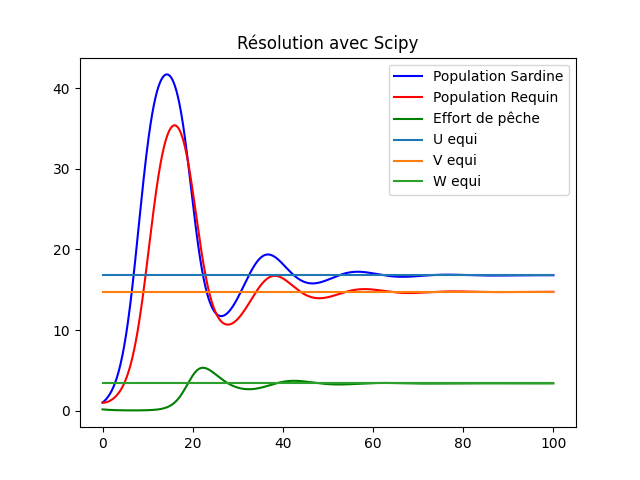
\includegraphics[width=7cm]{figures/Scipy_good_conditions.png}
            	\captionof{figure}{Évolution des grandeurs, méthode Scipy}
    		\end{minipage}
    		\hfill
    		\begin{minipage}[b]{.4\textwidth}
        		\centering
       			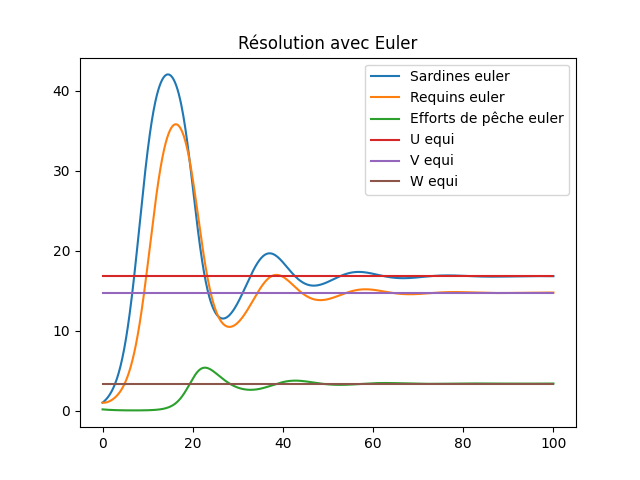
\includegraphics[width=7cm]{figures/Euler_good_conditions.png}
            	\captionof{figure}{Évolution des grandeurs, méthode d'Euler}
    		\end{minipage}
    		
		\end{figure}

        \begin{center}
            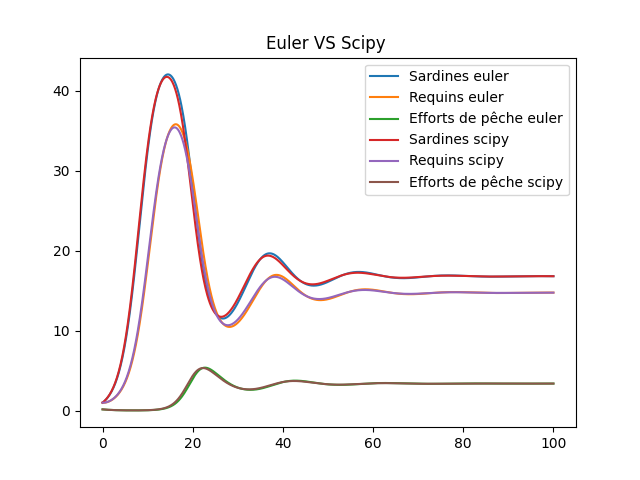
\includegraphics[width=8cm]{figures/Euler_VS_Scipy_good_conditions.png}
            \captionof{figure}{Comparaison des méthodes de résolution avec Euler explicite et Scipy}
        \end{center}

        % Courbes  : 3 portraits de phase 2d + ligne 3D u,v,w 
        \subsection{Portrait de phase des grandeurs $u,v,w$}
        Le graphique d'évolution de la population de requins, de la population de sardines et de l'effort de pêche est donné ci dessous.
         On remarque la convergence vers le point d'équilibre.
        \begin{center}
            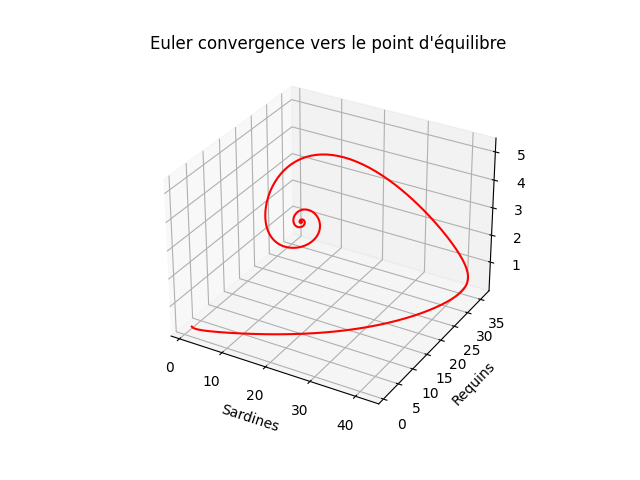
\includegraphics[width=8cm]{figures/convergence_3d_point_equilibre.png}
            \captionof{figure}{Convergence vers le point d'équilibre}
        \end{center}
        Les portraits de phases des 3 grandeurs sont ainsi obtenus.
        \begin{figure}[!h]
    		\begin{subfigure}[b]{.3\textwidth}
        		\centering
        		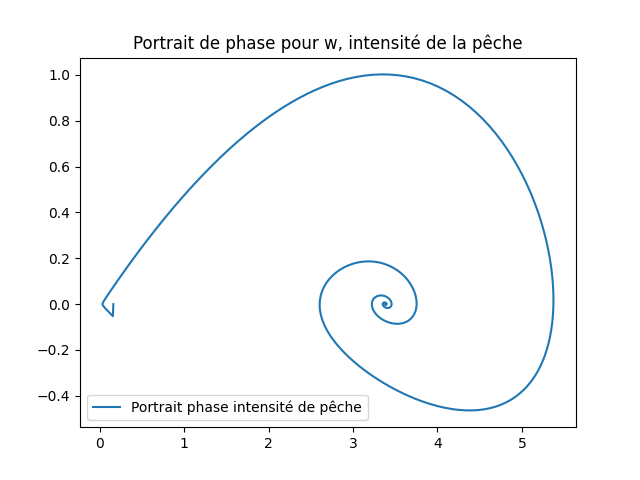
\includegraphics[width=\textwidth]{figures/Portrait_de_phase_peche.png}
            	\caption{Effort de pêche}
    		\end{subfigure}
    		\begin{subfigure}[b]{.3\textwidth}
        		\centering
       			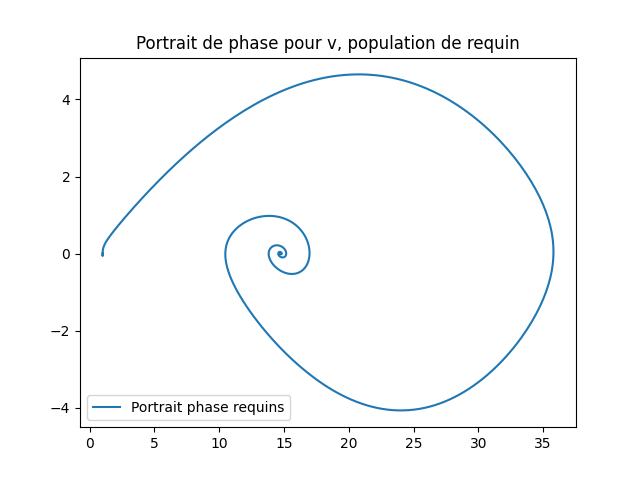
\includegraphics[width=\textwidth]{figures/Portrait_de_phase_requins.png}
            	%\captionof{figure}{Portrait de phase de la densité de requins}
        		\caption{Requins}
    		\end{subfigure}
    		\begin{subfigure}[b]{.3\textwidth}
        		\centering
       			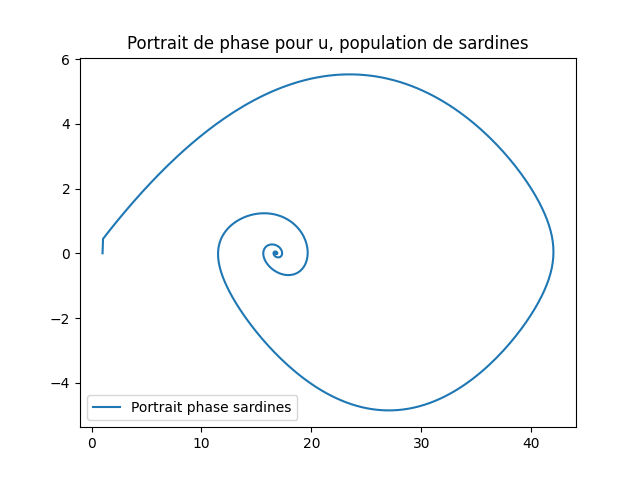
\includegraphics[width=\textwidth]{figures/Portrait_de_phase_sardine.png}
            	\caption{Sardines}
    		\end{subfigure}
    		\caption{Portrait de phases}
		\end{figure}


        % comparasion à nos attentes dans la vie réelle --> regarder les sardines disparaissent mer adriatique
        \subsection{Conclusion}
        On peut voir que notre modèle est juste, en effet on retrouve les résultats mis en exergue 
        dans les papiers de recherche à propos de ce sujet. On remarque également que nos modèles
        sont convergents, i.e. stable et consistant. De plus on remarque que la méthode de résolution avec
        scipy vient corroborer les résultats obtenus via la méthode d'euler explicite. Enfin, ces deux modèles
        permettent de vérifier nos intuitions quant aux dynamiques de population avec des cas particuliers,
        comme l'abscence de pêche qui induit un état d'équilibre plus haut pour la population de sardine. 
        Cependant les cas de ce genre ne sont pas exposés dans ce rapport par soucis de concision. 
        %\subsection{Cas particulier du système sans prédateur}

    \section{Modélisation à événements discrets}
        \subsection{Réseau de pétri}
        % Réseau de pétri 
        Pour modéliser la prise en compte des morts et naissances à l'état discret nous avons developper
        le modèle de Lotka-Volterra en temps discret avec le réseau de Pétri ci-dessous. 

        \begin{center}
            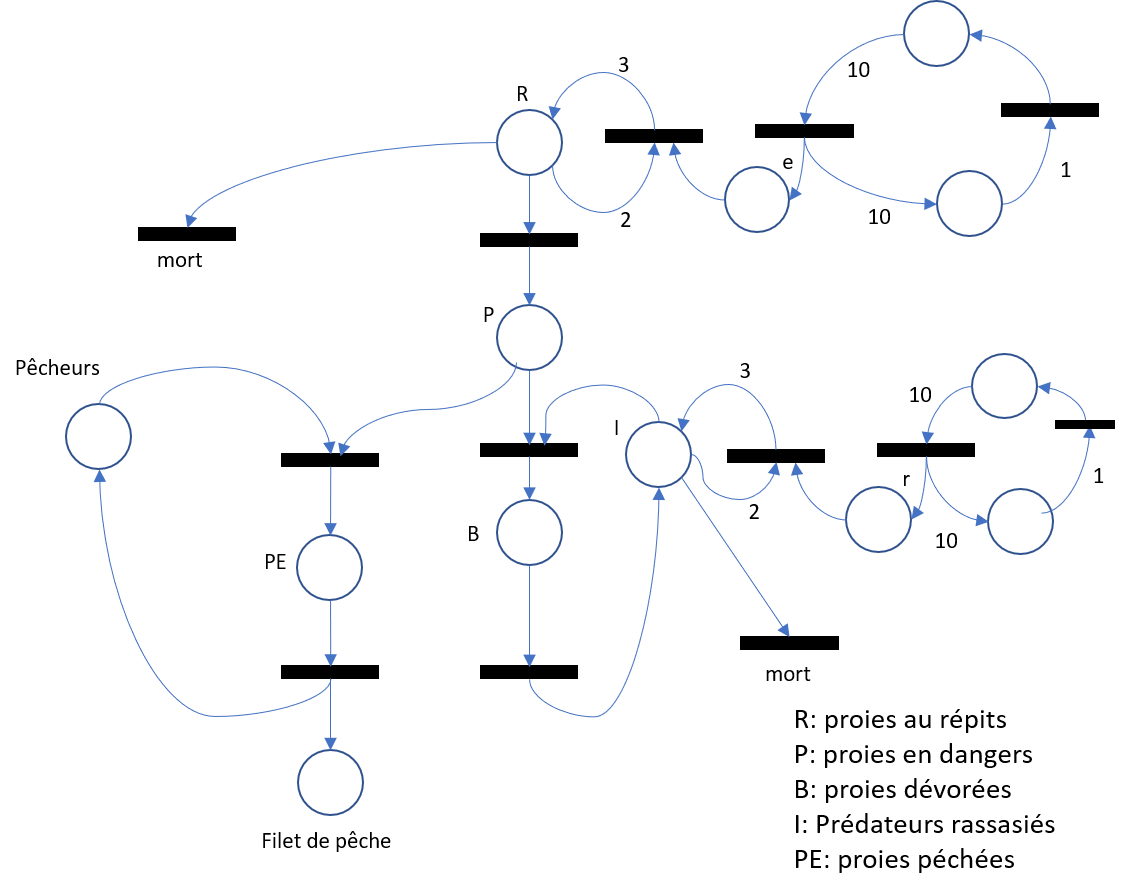
\includegraphics[width=15cm]{figures/reseau_petri.png}
            \captionof{figure}{Réseau de Pétri du système}
        \end{center}

        Ce réseau permet via un compteur de comptabilisé les paramètres $R_s$ et $R_r$  qui représentent les taux de
        reproduction des populations de sardines et de requins et $E_p$ qui permet de tenir compte del'effort de pêche . Il permet également via le même système de compteur de modéliser 
        l'effort de pêche. Aussi, la compétition entre individu définie par les variables $b_1$ et $b_2$ et pris en
        compte avec les puits qui symbolysent la mort d'un individu. 
    \section{Conclusion}
    Nous avons pu voir au terme de ce projet, les enjeux de la modélisation d'un phénomène complexe. En effet, 
    la prise d'initiative et d'hypothèses ont été primordiales afin de mener à bien notre projet de modélisation 
    de l'évolution des populations de sardines exposées à la pêche et à la chasse des requins en mer adriatique. 
    Par ailleurs, nous avons pu voir, par le biais de différentes modélisations, que les hypothèses changeaient
    en passant du temps discret au temps continu. Enfin nous pouvons affirmer que les résultats sont satisfaisants
    dans la mesure où ses derniers correspondent aux résultats mis en exergue dans les rapports de recherches emis 
    sur le sujet et dans la mesure où ils viennent corrober nos intuitions concernant la dynamique des populations.
    \nocite{*}
    \bibliographystyle{plain}
    \bibliography{biblio}% il faut un fichier .bib
\end{document}